\documentclass[pdf, aspectratio=169]{beamer}
\usepackage[]{hyperref,graphicx,siunitx,lmodern,booktabs,tikz,wasysym,caption}
\usepackage{pdfpc-commands}
\usepackage[mode=buildnew]{standalone}
\mode<presentation>{\usetheme{Astro}}

\sisetup{per-mode=symbol}
\usetikzlibrary{calc,angles,quotes}

\graphicspath{ {../Images/} }

%preamble
\title{Hitting the Elliptical}
\date{September 7, 2018}
\author{Jed Rembold}

\begin{document}
\renewcommand*{\theenumi}{\Alph{enumi}}

\begin{frame}{Announcements}
	\begin{itemize}
	  \item New WebWorK due Monday
	  \item Physics Tea today at 3pm!
	  \item I'm getting auctioned off as part of Phi Delta Theta's Ice Bucket Challenge fundraiser today around 5, so if you want to be part of dumping a bunch of ice water on me... give to the cause! :)
	  \item Poll: \url{rembold-class.ddns.net}
	\end{itemize}
\end{frame}

\begin{frame}{Observing Events Tonight}
	\begin{columns}
		\column{0.5\textwidth}
		\begin{itemize}
			\item Neptune at opposition today!
			\item Venus and Jupiter also visible low in the west after sunset
			\item Mars visible to the southeast
			\item Saturn to the south
		\end{itemize}
		
		\column{0.5\textwidth}
		\begin{center}
			\includegraphics[width=.9\textwidth]{20180907PlanetsToday.png}
		\end{center}
		
	\end{columns}
\end{frame}

\begin{frame}{Review Question}
  \begin{columns}
	\column{.5\textwidth}
	The picture to the right was supposedly taken in Sydney (\SI{33.9}{\degree S}, \SI{151.4}{\degree E}), and shows the classic star trails of a prolonged exposure. What is wrong with it?
	\begin{enumerate}
	  \item There is no moon in the image
	  \item \alert<2>{The pole is too low in the sky}
	  \item The stars are spinning the wrong direction
	  \item There is nothing wrong with it!
	\end{enumerate}
	\column{.5\textwidth}
	\begin{figure}[h!]
	  \centering
	  \includegraphics[width=\textwidth]{ch3_BadSydneySky.png}
	\end{figure}
  \end{columns}
\end{frame}

\begin{frame}[fragile]{A Corrected Geocentric Model: Ptolemy}
  \begin{center}
	\begin{tikzpicture}
	  \newcommand{\orbit}[3]{
		\draw[dashed, #1, -latex] (#2,0) arc (0:90:#2cm);
		\coordinate (p) at (#3:#2);
		\draw[dotted, #1, -latex] (p) +(0:4mm) arc(0:340:4mm);
		\fill[#1] (p) +(0:4mm) circle(1mm);
	  }
	  \node at (0,0) {\includegraphics[width=1cm]{world.png}};
	  \orbit{red!50}{1}{0};
	  \orbit{yellow!50}{2}{20};
	  \orbit{yellow}{3}{30};
	  \orbit{black!10!red}{4}{40};
	  \orbit{red}{5}{50};
	  \orbit{black!10!yellow}{6}{60};
	\end{tikzpicture}
  \end{center}
\end{frame}

\begin{frame}{The Ptolemaic Model ($\approx$ 150 AD)}
  \begin{itemize}
	\item The basic Aristotle idea of the geocentric model is very simple
	\item In practice though, the Ptolemaic model is actually extremely complex
	  \begin{itemize}
		\item Some circles larger than others
		\item Some circles slightly rotating off-center
	  \end{itemize}
	\item It DID, however, quite accurately predict the observed motion of the planets
  \end{itemize}
\end{frame}

\begin{frame}{Enter Copernicus (1473-1543)}
  \begin{itemize}
	\item Found that the planetary motion tables based on Ptolemaic model were growing more inaccurate
	\item Disliked the complexity of Ptolemaic model on aesthetic grounds
	\item Adopted a \alert{heliocentric} model with the Sun at the center
	  \begin{itemize}
		  \item Naturally explains retrograde motion \href{http://physics.unm.edu/Courses/Rand/applets/retrograde.html}{\textcolor{orange}{(See here)}}
		\item Naturally explained Mercury and Venus never being a large angle from the Sun
	  \end{itemize}
	\item The Heliocentric model was \alert{not} significantly more accurate than the Ptolemaic model at the time.
  \end{itemize}
\end{frame}

\begin{frame}{Objection! The Church}
  \begin{quote}
	There is talk of a new astrologer who wants to prove that
the earth moves and goes around, instead of the sky,
the sun, the moon, just as if somebody were moving in a
carriage or ship might hold that he was sitting still and at
rest while the earth and the trees walked and moved.
But that is how things are nowadays: when a man
wishes to be clever he must needs invent something
special, and the way he does it must needs be the best!
The fool wants to turn the whole art of astronomy
upside-down. However, as Holy Scripture tells us, so did
Joshua bid the sun to stand still and not the earth. 
  \end{quote}
  \begin{flushright}
	-Martin Luther
  \end{flushright}
\end{frame}

\begin{frame}{Objection! Science}
  \begin{columns}
	\column{.5\textwidth}
	\begin{itemize}
	  \item Why aren't we dizzy?
	  \item Why are we the only planet with a moon?
	  \item Why don't we see stellar parallax?
	\end{itemize}
	\column{.5\textwidth}
	\begin{center}
	  \begin{tikzpicture}[scale=0.9]
		\draw[inner color=yellow, outer color=orange] (0,0) circle(2mm);
		\draw[dashed] (0,0) circle (1.5cm);
		\draw[dashed] (0,0) circle (3cm);
		\coordinate (e2) at (330:1.5);
		\coordinate (e1) at (180:1.5);
		\node at (e1) {\includegraphics[width=2mm]{world.png}};
		\node at (e2) {\includegraphics<3->[width=2mm]{world.png}};
		\foreach \a in {0,20,...,340}{
		  \node (\a) at (\a:3) {$\bigstar$};
		}
		\fill<2->[cyan, fill opacity=0.4] (180)--(e1)--(220);
		\fill<3->[orange, fill opacity=0.4] (180)--(e2)--(220);
	  \end{tikzpicture}
	\end{center}
  \end{columns}
\end{frame}

\begin{frame}{Tycho Brahe (1546-1601)}
  \begin{columns}
	\column{.5\textwidth}
	\begin{itemize}
	  \item Last real ``naked-eye'' astronomer
	  \item Took very precise angle measurements of stars and planets
	  \item Saw no stellar parallax, and thus thought Copernicus wrong
	  \item Hired Kepler as assistant
	\end{itemize}
	\column{.5\textwidth}
	\begin{center}
	  \includegraphics[width=\textwidth, height=.9\textwidth, keepaspectratio]{ch3_brahe.jpg}
	\end{center}
  \end{columns}
\end{frame}

\begin{frame}{Johannes Kepler (1571-1630)}
  \begin{itemize}
	\item Spent 8 years trying to reconcile Tycho's Mars observations with the Ptolemaic model
  \end{itemize}
  \begin{quotation}
	Who would have thought it possible? This
hypothesis, which so closely agrees with the
observed oppositions, is nevertheless false? If I
had believed that we could ignore those 8 minutes, I
would have patched up my hypothesis accordingly.
But since it was not possible to ignore them,
those 8 minutes point the road to a complete
reform of astronomy\ldots

Thou seest now, diligent reader, that the hypothesis
based on this method not only satisfies the four
positions on which it was based, but also
correctly represents within 2 minutes all the
other observations. 
  \end{quotation}
  \begin{flushright}
	- Johannes Kepler, \underline{Nova Astronomica}
  \end{flushright}
\end{frame}

\begin{frame}{Kepler's 1st Law}
  \begin{itemize}
	\item The orbits of the planets are ellipses
	  \begin{itemize}
		\item The Sun at one focus and \alert{nothing} at the other
	  \end{itemize}
  \end{itemize}
  \begin{center}
	\begin{tikzpicture}
	  \def\a{4}
	  \def\b{3}
	  \draw (0,0) ellipse (\a cm and \b cm);
	  \node[draw,fill,circle, inner sep=1pt,label={below:Nothing}] (f1) at ({-sqrt(\a*\a-\b*\b)},0) {};
	  \node[fill,circle, inner sep=3pt, inner color=yellow, outer color=orange,label={below:Sun}] (f2) at ({sqrt(\a*\a-\b*\b)},0) {};
	  \node at ($(0,0)+(45:{\a} and {\b})$) {\includegraphics[width=3mm]{world.png}};
	\end{tikzpicture}
  \end{center}
\end{frame}

\begin{frame}{Ellipses}
  \begin{itemize}
	\item Look like squished circles
	\item Described by:
	  \begin{itemize}
		\item<1-> Major Axis (longest width)
		\item Eccentricity (squished-ness)
	  \end{itemize}
	  \begin{center}
		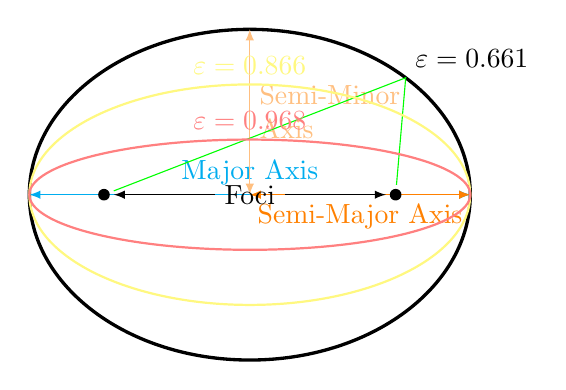
\begin{tikzpicture}[scale=0.7]
		  \draw[very thick] (0,0) ellipse (4cm and 3cm);
		  \draw<1>[latex-latex,cyan] (-4,0) -- node[midway,above] {Major Axis}(4,0);
		  \draw<2>[latex-latex, orange] (0,0) -- node[midway,below] {Semi-Major Axis} (4,0);
		  \draw<3>[latex-latex, orange!50] (0,0) -- node[midway,right, align=left] {Semi-Minor\\Axis} (0,3);
		  \onslide<4>{
			\fill ({sqrt(4*4-3*3)},0) node (f1) {} circle (3pt);
			\fill ({-sqrt(4*4-3*3)},0) node (f2) {} circle (3pt);
			\node (flab) at (0,0) {Foci};
			\draw[-latex] (flab) -- (f1);
			\draw[-latex] (flab) -- (f2);
			\coordinate (a) at ($(0,0)+(45:4cm and 3cm)$);
			\coordinate (b) at ($(0,0)+(195:4cm and 3cm)$);
			\draw[green] (f1) -- (a) -- (f2);
		  }
		  \onslide<5>{
			\node[above right] at (a) {$\varepsilon=0.661$};
			\draw[thick, yellow!50] (0,0) ellipse (4cm and 2cm);
			\node[above,yellow!50] at (0,2) {$\varepsilon=0.866$};
			\draw[thick, red!50] (0,0) ellipse (4cm and 1cm);
			\node[above,red!50] at (0,1) {$\varepsilon=0.968$};
		  }
		\end{tikzpicture}
	  \end{center}
	\item<5> A circle is an ellipse with eccentricity=0
  \end{itemize}
\end{frame}

\begin{frame}{Ellipse Math}
  You can always get the foci location and eccentricity from the semi-major and minor axes.
  \begin{columns}
	\column{.4\textwidth}
	\begin{itemize}
	  \item Foci:
		\[f = \sqrt{a^2-b^2}\]
	  \item Eccentricity:
		\[\varepsilon = \sqrt{1-\frac{b^2}{a^2}}\]
	  \item Area:
		\[A = \pi a b\]
	\end{itemize}
	\column{.6\textwidth}
	\begin{center}
	  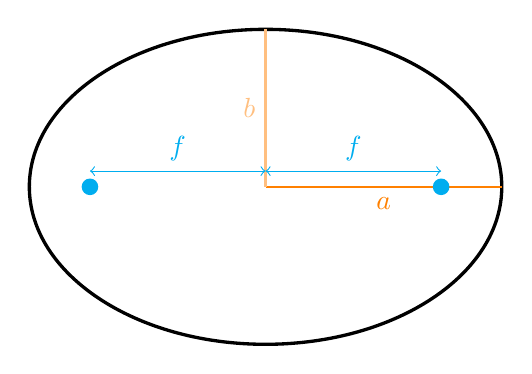
\begin{tikzpicture}
		\draw[very thick] (0,0) ellipse (3cm and 2cm);
		\draw[orange, thick] (0,0) -- node[midway,below] {$a$} (3,0);
		\draw[orange!50, thick] (0,0) -- node[midway,left] {$b$} (0,2);
		\fill[cyan] (2.23,0) circle (3pt);
		\draw[<->, cyan] (0,0.2) -- node[midway,above] {$f$} (2.23,0.2);
		\fill[cyan] (-2.23,0) circle (3pt);
		\draw[<->, cyan] (0,0.2) -- node[midway,above] {$f$} (-2.23,0.2);
	  \end{tikzpicture}
	\end{center}
  \end{columns}
\end{frame}

\begin{frame}{Elliptical Orbits}
  \begin{itemize}
	\item Most Solar System orbits are not particularly eccentric
	  \begin{itemize}
		\item Look pretty circular
		\item<4> Sun is NOT at center however
	  \end{itemize}
  \end{itemize}
  \begin{center}
	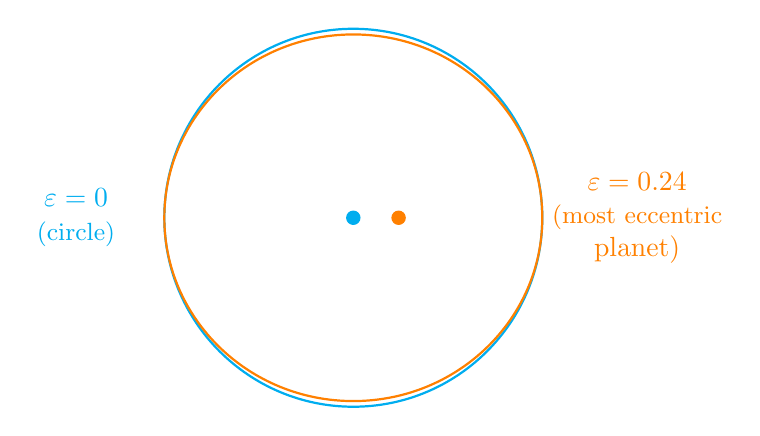
\begin{tikzpicture}[scale=.8]
	  \draw<1,3->[thick,cyan] (0,0) circle (3cm);
	  \node<1,3->[left,align=center,cyan,xshift=-5mm] at ($(0,0)+(180:3)$) {$\varepsilon=0$\\\small(circle)};
	  \draw<2,3->[thick,orange] (0,0) ellipse (3cm and 2.91cm);
	  \node<2,3->[right,align=center,orange] at ($(0,0)+(0:3)$) {$\varepsilon=0.24$\\\small(most eccentric\\ planet)};
	  \draw<4>[fill,cyan] (0,0) circle (3pt);
	  \draw<4>[fill,orange] (0.719,0) circle (3pt);
	\end{tikzpicture}
  \end{center}
\end{frame}

\begin{frame}{Understanding Check!}
  Why of the following depicts a possible planet orbit?
  \begin{center}
	\hspace{5mm}
	\begin{tikzpicture}[sun/.style={inner color=yellow, outer color=orange},scale=0.5]
	  \draw (0,0) ellipse (4cm and 2.5cm);
	  \fill[sun] (0,0) circle (5mm);
	  \node at ($(0,0)+(45:4 and 2.5)$) {\includegraphics[width=2mm]{world.png}};
	  \node at (0,1.5) {\LARGE A};
	\end{tikzpicture}\hspace{5mm}
	\begin{tikzpicture}[sun/.style={inner color=yellow, outer color=orange},scale=0.5]
	  \draw (0,0) ellipse (4cm and 2.5cm);
	  \fill[sun] (3.1,0) circle (5mm);
	  \node at ($(0,0)+(125:4 and 2.5)$) {\includegraphics[width=2mm]{world.png}};
	  \node at (0,1.5) {\LARGE B};
	\end{tikzpicture}\vspace{5mm}
	\begin{tikzpicture}[sun/.style={inner color=yellow, outer color=orange},scale=0.5]
	  \draw (0,0) ellipse (4cm and 2.5cm);
	  \fill[sun] (-5,0) circle (5mm);
	  \node at ($(0,0)+(225:4 and 2.5)$) {\includegraphics[width=2mm]{world.png}};
	  \node at (0,1.5) {\LARGE C};
	\end{tikzpicture}\hspace{5mm}
	\begin{tikzpicture}[sun/.style={inner color=yellow, outer color=orange},scale=0.5]
	  \draw (0,0) ellipse (4cm and 2.5cm);
	  \fill[sun] (0,-1.5) circle (5mm);
	  \node at ($(0,0)+(325:4 and 2.5)$) {\includegraphics[width=2mm]{world.png}};
	  \node at (0,1.5) {\LARGE D};
	\end{tikzpicture}
  \end{center}
\end{frame}

\begin{frame}{Kepler's 2nd Law}
  \begin{itemize}
	\item A line joining a planet to the sun sweeps out equal areas in equal times
	  \begin{itemize}
		\item Planets move faster when close to the Sun and slower when far away
	  \end{itemize}
  \end{itemize}
  \begin{center}
	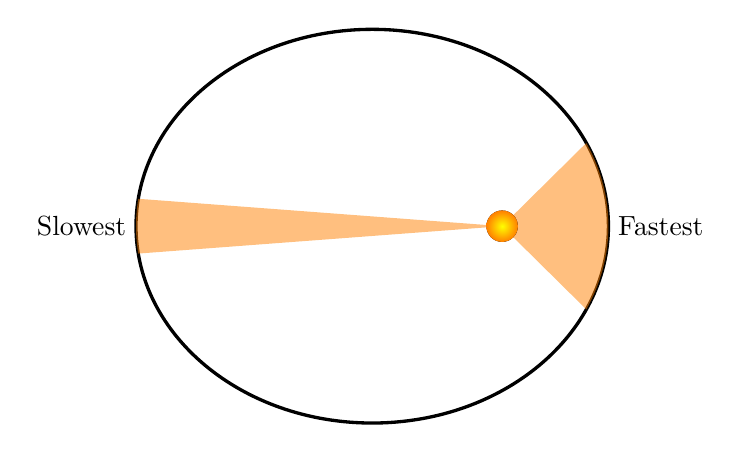
\begin{tikzpicture}
	  \coordinate (sun) at (1.65,0);
	  \draw[very thick] (0,0) ellipse (3cm and 2.5cm);
	  \fill[opacity=0.5,orange] (sun) -- (-25:3cm and 2.5cm) arc (-25:25:3cm and 2.5cm);
	  \fill[opacity=0.5,orange] (sun) -- (172:3cm and 2.5cm) arc (172:188:3cm and 2.5cm);
	  \fill[inner color=yellow, outer color=orange] (sun) circle (2mm);
	  \node[right] at (3,0) {Fastest};
	  \node[left] at (-3,0) {Slowest};
	\end{tikzpicture}
  \end{center}
\end{frame}

\begin{frame}{Kepler's 3rd Law}
  \begin{itemize}
	\item The square of a planet's orbital period is proportional to the cube of its semi-major axis.
	  \begin{itemize}
		\item A planet's \alert{period} is the time it takes to complete an entire orbit
		\item An orbit's semi-major axis we defined earlier to be half the major axis
	  \end{itemize}
	\item Mathematically, this looks like
	  \[p^2 \propto a^3\]
	  where $p$ is the period and $a$ is the semi-major axis
	\item If you measure period in years and the semi-major axis in AU, then
	  \[p^2 \approx a^3\]
  \end{itemize}
\end{frame}

\begin{frame}{Example!}
  The below image is the orbit of some astronomical object. Each grid is \SI{1}{AU} in length. Determine:
  \begin{enumerate}
	\item Where the Sun is located. \onslide<2->{\color{LOrange}At one of the foci\color{fg}}
	\item What the orbital period is. \onslide<3->{\color{LOrange}8 years\color{fg}}
	%\item Approximately where the object is in 3 years. \onslide<4->{\color{LOrange}$\approx$\SI{4.7}{A\square U\per yr}\color{fg}}
  \end{enumerate}
  \begin{center}
	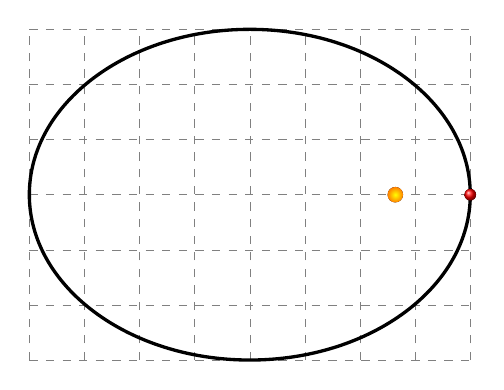
\begin{tikzpicture}[scale=0.7]
	  \draw[help lines, dashed] (-4,-3) grid (4,3);
	  \draw[very thick] (0,0) ellipse (4cm and 3cm);
	  \fill[ball color=red] (4,0) circle (3pt);
	  \fill<2->[inner color=yellow, outer color=orange] (2.64,0) circle (4pt);
	  %\fill<4->[red!50,opacity=0.5] (4,0) -- (2.64,0) -- (150:4 and 3) arc (150:0:4 and 3);
	\end{tikzpicture}
  \end{center}
\end{frame}

%\begin{frame}[t]{Enter Galileo!}
  %\begin{columns}[t]
	%\column{.45\textwidth}
	%\begin{block}{Kepler}
	  %\begin{itemize}
		%\item Derived entirely from Brahe's naked eye observations
		%\item Only ``proof'' was that they explain everything nice and simple
	  %\end{itemize}
	%\end{block}
	%\column{.45\textwidth}
	%\begin{block}{Galileo}
	  %\begin{itemize}
		%\item Strongly believed in Copernicus's heliocentric solar system
		%\item Wanted to \emph{prove} that the Earth orbited the Sun
		%\item Did not \emph{invent} the telescope, but was almong the first to use it to study the heavens
		%\item Widely published his findings
	  %\end{itemize}
	%\end{block}
  %\end{columns}
%\end{frame}

%\begin{frame}{The Observations of Galileo}
  %\begin{center}
	%\begin{tikzpicture}
	  %\begin{scope}
		%\clip (0,0) rectangle (5,7);
		%\node[anchor=south west] at (0,0) {\includegraphics[width=10cm]{ch4_gal_moons.jpg}};
	  %\end{scope}
	  %\node[anchor=south west] at (5,2.5) {\includegraphics[width=4.3cm]{ch4_gal_moon.png}};
	  %\node[anchor=south west] at (5,0) {\includegraphics[width=5cm]{ch4_gal_phases.jpg}};
	%\end{tikzpicture}
  %\end{center}
%\end{frame}

%\begin{frame}{Sunspots!}
  %\begin{figure}[h!]
	%\centering
	%\includegraphics[width=.7\textwidth, height=.5\textwidth, keepaspectratio]{ch4_gal_sunspots.png}
  %\end{figure}
%\end{frame}

%\begin{frame}{More Modern Phases of Venus}
  %\begin{figure}[h!]
	%\centering
	%\includegraphics[width=\textwidth]{ch4_venus_phase.jpg}
  %\end{figure}
%\end{frame}

%\begin{frame}{The Physics of Galileo!}
  %\begin{columns}
	%\column{.5\textwidth}
	%\begin{itemize}
	  %\item Disputed ``classical'' Aristotle physics
	  %\item Made large strides in how we think about:
		%\begin{itemize}
		  %\item<2-> Relative Motion
		  %\item<3-> Inertia
		  %\item<4-> Falling bodies
		  %\item<5-> Projectiles
		%\end{itemize}
	%\end{itemize}
	%\column{.5\textwidth}
	%\begin{figure}[h!]
	  %\centering
	  %\includegraphics<4>[width=.8\textwidth, height=.8\textwidth, keepaspectratio]{ch4_pisa.jpg}
	  %\includegraphics<5>[width=\textwidth]{ch4_gal_projectile.png}
	  %\includegraphics<2>[width=\textwidth]{ch4_gal_relmot.jpg}
	  %\includegraphics<3>[width=\textwidth]{ch4_gal_incline.jpg}
	%\end{figure}
  %\end{columns}
%\end{frame}

%%\begin{frame}{Galileo's Relativity}
  %%\begin{quotation}
	%%Shut yourself up with some friend in the main cabin below decks on some large ship, and have with you there some flies, butterflies, and other small flying animals. Have a large bowl of water with some fish in it; hang up a bottle that empties drop by drop into a wide vessel beneath it\ldots
	
	%%When you have observed all these things carefully\ldots have the ship proceed with any speed you like, so long as the motion is uniform and not fluctuating this way and that.
	
	%%\alert{You will discover not the least change in all the effects named, nor could you tell from any of them whether the ship was moving or standing still.}
  %%\end{quotation}
%%\end{frame}

%%\begin{frame}{Inertia}
  %%\begin{itemize}
	%%\item Aristotle thought: \emph{A body at rest tends to remain at rest}
	%%\item Galileo extended this to be:
	  %%\begin{center}
		%%\alert{A body at rest tends to remain at rest.}\\
		%%AND\\
		%%\alert{A body in motion tends to remain in motion.}
	  %%\end{center}
	%%\item This is the idea of \underline{inertia}, developed further by Newton
  %%\end{itemize}
  %%\begin{center}
	%%\begin{tikzpicture}
	  %%\coordinate (o) at (0,0);
	  %%\draw[thick, fill] (0,0) -- ++(3,0) -- ++(30:4) coordinate (a) -- (o-|a);
	  %%\fill[ball color=orange,yshift=6pt] ($(3,0)+(30:3)$) circle (5pt);
	  %%\fill[ball color=orange,yshift=6pt] ($(3,0)+(30:2)$) circle (5pt);
	  %%\fill[ball color=orange,yshift=6pt] ($(3,0)+(30:1)$) circle (5pt);
	  %%\fill[ball color=orange,yshift=6pt] (2,0) node (ball) {} circle (5pt);
	  %%\node[fill=Blue, rounded corners,align=center, text=black] (box) at (1,2) {Ball will keep\\rolling without\\friction};
	  %%\draw[-latex,Blue] (box.south) -- (ball);
	%%\end{tikzpicture}
  %%\end{center}
%%\end{frame}

%%\begin{frame}{Falling Bodies}
  %%\begin{columns}
	%%\column{.5\textwidth}
	%%\begin{center}
	  %%\begin{tikzpicture}[scale=0.9, transform shape]
		%%\shade[top color=LBlue, bottom color=Blue2, rounded corners] (0,0) rectangle (5,7);
		%%\node[anchor=south west] at (0,0) {\includegraphics[width=1.5cm]{ch4_pisa.pdf}};
		%%\fill[ball color=Blue2] (2,1) circle (3pt);
		%%\fill[ball color=Orange] (2.4,1) circle (5pt);
		%%\node[anchor=south west,xscale=-1] at (5,2.7) {\includegraphics[width=1.5cm]{ch4_pisa.pdf}};
		%%\fill[ball color=Blue2] (3,5) circle (3pt);
		%%\fill[ball color=Orange] (2.8,4) circle (5pt);
		%%\node[text=black] at (2.5,6) {Aristotle};
		%%\node[text=black] at (3,0.5) {Galileo};
	  %%\end{tikzpicture}
	%%\end{center}
	%%\column{.5\textwidth}
	%%\begin{itemize}
	  %%\item Galileo's experiments convinced him that object fall at same rate w/o air resistance
	  %%\item A feather and chunk of lead fall at the same speed in a vaccuum!
	%%\end{itemize}
  %%\end{columns}
%%\end{frame}

%\begin{frame}{Kepler and Galileo}
  %\begin{columns}
	%\column{.5\textwidth}
	%\begin{itemize}
	  %\item Around during the same time period
		%\begin{itemize}
		  %\item Keplers first Laws published in 1609
		  %\item Galileo's first telescope observations 1610
		%\end{itemize}
	  %\item Despite church resistance, the heliocentric model gain acceptance over the next 50 years
	%\end{itemize}
	%\column{.5\textwidth}
	%\begin{center}
	  %\begin{tikzpicture}
		%\onslide<1>{
		  %\node (img) at (0,0) {\includegraphics[width=.5\textwidth]{ch4_kepler.jpg}};
		  %\node[below] at (img.south) {Kepler: 1571-1630};
		%}
		%\onslide<2>{
		  %\node (img) at (0,0) {\includegraphics[width=.5\textwidth]{ch4_galileo.jpg}};
		  %\node[below] at (img.south) {Galileo: 1564-1642};
		%}
	  %\end{tikzpicture}
	%\end{center}
  %\end{columns}
%\end{frame}

%\begin{frame}{Good Sir Isaac}
  %\begin{columns}
	%\column{.5\textwidth}
	%\begin{figure}[h!]
	  %\centering
	  %\includegraphics[width=.6\textwidth]{ch4_isaac.jpg}
	  %\caption*{Isaac Newton: 1642-1727}
	%\end{figure}
	%\column{.5\textwidth}
	%\begin{itemize}
	  %\item Was able to relate the behavior of orbiting bodies to the behavior of bodies on Earth
	  %\item Short and Succinct: Summarized everything in four sentences\ldots
	%\end{itemize}
  %\end{columns}
%\end{frame}

%\begin{frame}{Newton's First Law}
  %\begin{alertblock}{Newton's First Law}
	%A body continues in a state of rest or uniform motion in a straight line unless acted on by a force.
  %\end{alertblock}
  %\begin{itemize}
	%\item Implications for astronomy?
	  %\begin{itemize}
		%\item A object that falls when released must be feeling a force
		%\item An object moving in a circle must have a force acting upon it, else it would travel in a straight line
	  %\end{itemize}
	%\item Generally thought of as the inertia law
  %\end{itemize}
%\end{frame}

%\begin{frame}{Newton's Second Law}
  %\begin{alertblock}{Newton's Second Law}
	%The force on an object is equal to the mass of the object multiplied by its acceleration.
	%\[\scalebox{4}{F = ma}\]
  %\end{alertblock}
  %\begin{itemize}
	%\item An acceleration is analogous to a change in motion
	%\item Such a change in motion depends only on the force applied and the mass of the object
	%\item \alert{The change in motion is in the same direction as the force!}
  %\end{itemize}
%\end{frame}

%\begin{frame}{Force Examples}
  %\begin{columns}
	%\column{.5\textwidth}
	%\begin{figure}[h!]
	  %\centering
	  %\begin{tikzpicture}
		%\node[fill, ball color=red, circle] (ball1) at (0,0) {};
		%\draw[thick, green, -latex] (ball1) --+(0,-0.5);
		%\node[fill, ball color=red, circle] (ball2) at (1,-.5) {};
		%\draw[thick, green, -latex] (ball2) --+(0,-1.5);
		%\draw[thick, orange, -latex] (-0.5,0) -- node[midway,sloped,below] {Force} (-0.5, -2);
	  %\end{tikzpicture}
	  %\caption*{A ball dropping must feel a force to accelerate downwards!}
	%\end{figure}
	%\column{.5\textwidth}
	%\begin{figure}[h!]
	  %\centering
	  %\begin{tikzpicture}
		%\node[fill, ball color=red, circle] (ball1) at (0,2) {};
		%\draw[thick, green, -latex] (ball1) arc (90:10:2cm);
		%\node[fill, ball color=red, circle] (ball1) at (0,2) {};
		%\draw[thick, orange, -latex] (45:2cm) -- node[midway,sloped,below] {Force} (0,0);
	  %\end{tikzpicture}
	  %\caption*{A ball curving at a constant speed must still feel a force turning it!}
	%\end{figure}
  %\end{columns}
%\end{frame}

%\begin{frame}{Circular Motion}
  %\begin{itemize}
	%\item Of particular interest to us is circular motion, since such motion largely describes the motion of the planets
	%\item Newton tells us that, even if our planets are moving at a constant speed, a force \alert{must} be present to keep them moving in a circular orbit
	  %\begin{center}
		%\begin{tikzpicture}[scale=0.7]
		  %\fill[inner color=yellow, outer color=orange] (0,0) circle (1cm);
		  %\draw[dashed, -latex, thick] (3,0) arc (0:340:3cm);
		  %\onslide<2->{
			%\foreach \a in {0,45,...,350}{
			  %\draw[orange, -latex] (\a:2.7) -- (\a:1.3);
			%}
		  %}
		  %\node at (3,0) {\includegraphics[width=1cm]{world.png}};
		  %\onslide<3>{\node[fill=Blue2, rounded corners, text=fg, align=center, anchor=west] at (4,-2) {But what is this\\regulating force?};}
		%\end{tikzpicture}
	  %\end{center}
  %\end{itemize}
%\end{frame}

%\begin{frame}{Sup G?}
  %\begin{itemize}
	%\item Gravity! The universal attractor
	  %\begin{itemize}
		%\item Anything with mass attracts anything else with mass
		%\item Strength of force depends on the masses involved
		%\item Strength of the force diminished rapidly with distance
	  %\end{itemize}
  %\end{itemize}
  %\begin{center}
	%\begin{tikzpicture}
	  %\coordinate (ball1) at (0,0);
	  %\coordinate (ball2) at (8,0);
	  %\coordinate (d) at ($(ball1)-(0,1.5)$);
	  %\draw[green] (ball1) --+(0,-2);
	  %\draw[cyan] (ball2) --+(0,-2);
	  %\fill[ball color=green] (ball1) circle (1cm);
	  %\fill[ball color=cyan] (ball2) circle (1cm);
	  %\node at ($(ball1)+(0,1.2)$) {$M_1$};
	  %\node at ($(ball2)+(0,1.2)$) {$M_2$};
	  %\draw[<->, thick] (d) -- node[midway,below] {d} (d-|ball2);
	  %\draw[-latex, ultra thick,orange] (ball1) -- +(4,0);
	  %\draw[-latex, ultra thick,orange] (ball2) -- +(-4,0);
	  %\node[orange] at (4,1) {\scalebox{1.5}{$F_g = G \frac{M_1 M_2}{d^2}$}};
	%\end{tikzpicture}
  %\end{center}
%\end{frame}

%\begin{frame}{Gravitational Force on You!}
  %\begin{example}
	%Let's find the force of gravity between you, an average \SI{70}{\kilo\gram} individual, and the Earth, with its \SI{5.97E24}{\kilo\gram} mass. The Earth has an average radius of \SI{6378}{\kilo\meter}. What acceleration do you experience?
	%\onslide<2->{
	  %\[F_g = (\SI{6.67E-11}{})\frac{(\SI{5.97E24}{})(70)}{(6378000)^2} = \SI{685.2}{\newton}\]
	%}
	%\onslide<3->{
	  %\[F_g = ma = \SI{685.2}{\newton} = (70)a \quad\Rightarrow a = \SI{9.79}{\meter\per\second^2}\]
	%}
  %\end{example}
%\end{frame}

%\begin{frame}{The Fine Art of Throwing Things}
  %\begin{itemize}
	%\item Say you throw a ball sideways
	  %\begin{itemize}
		%\item<2-> You force the ball (using your arm) up to some speed
		%\item<3-> Inertia keeps the ball moving forward at that speed
		%\item<4-> Gravity drags the ball down
	  %\end{itemize}
  %\end{itemize}
  %\begin{center}
	%\begin{tikzpicture}
	  %\node at (0,0) {\includegraphics[width=3cm]{ch4_thrower.pdf}};
	  %%\fill[ball color=orange] (0,0) circle (3pt);
	  %\onslide<1>{\fill[ball color=green] (115:1.5) coordinate (p1) circle (3pt);}
	  %\onslide<2>{
		  %\fill[ball color=green] ($(p1)+(1,0)$) coordinate (p2) circle (3pt);
		%\draw[orange, thick,-latex] (p1) -- +(.9,0);
	  %}
	  %\onslide<3>{
		%\fill[ball color=green] ($(p2)+(1,0)$) circle (3pt);
	  %}
	  %\onslide<4>{
		%\foreach[count=\x] \y in {1.8,1.5, 0.9, 0.2, -.6, -1.5}{
		  %%\fill[ball color=green, opacity=\x/6] (2+\x,\y) circle (3pt);
		  %\fill[ball color=green, opacity=\x/6] ($(p2)+(\x+1,{\y-1.8})$) circle (3pt);
		%}
	  %}
	%\end{tikzpicture}
  %\end{center}
%\end{frame}

%\begin{frame}{One Powerful Arm\ldots}
  %\begin{itemize}
	%\item Now, if we hiked up a tall mountain and had a REALLY REALLY strong arm\ldots
	%\item \href{http://galileoandeinstein.physics.virginia.edu/more_stuff/flashlets/NewtMtn/home.html}{Newton's Mountain}
  %\end{itemize}
%\end{frame}

\end{document}
